Neben den beiden selbst erzeugten Szenarien, werden nun Szenarien betrachtet, in denen die Terrain-Generierung der Blocklib genutzt wird. Für die Generierung nutzt die Blocklib einen Pseudo-Zufallszahlengenerator. Das ist ein Algorithmus, der ausgehend von einem übergebenen Wert, dem sogenannten \emph{Seed} Werte erzeugt, die zufällig wirken. Der Algorithmus ist allerdings deterministisch. Mit demselben Seed wird immer dieselbe Folge von Zahlen generiert.

\begin{figure}
	\centering
	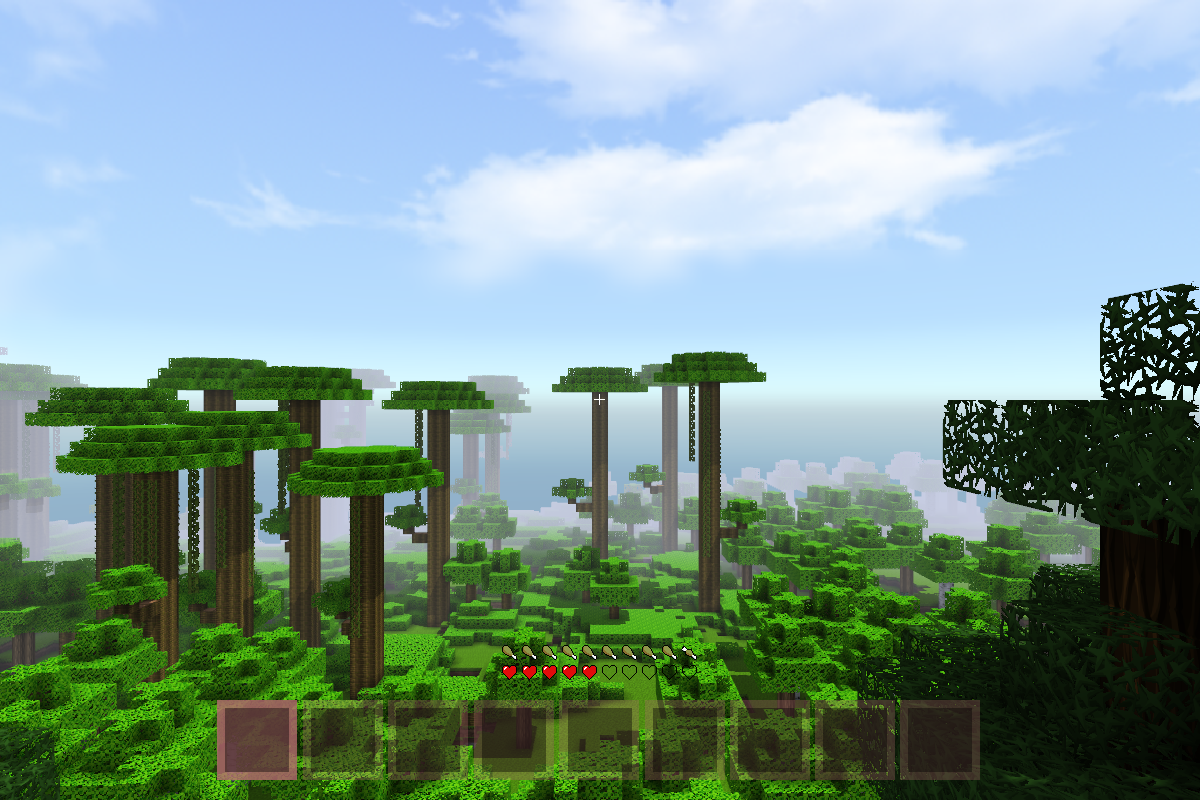
\includegraphics[width=.49\textwidth]{seed-0.png}
	\hfill
	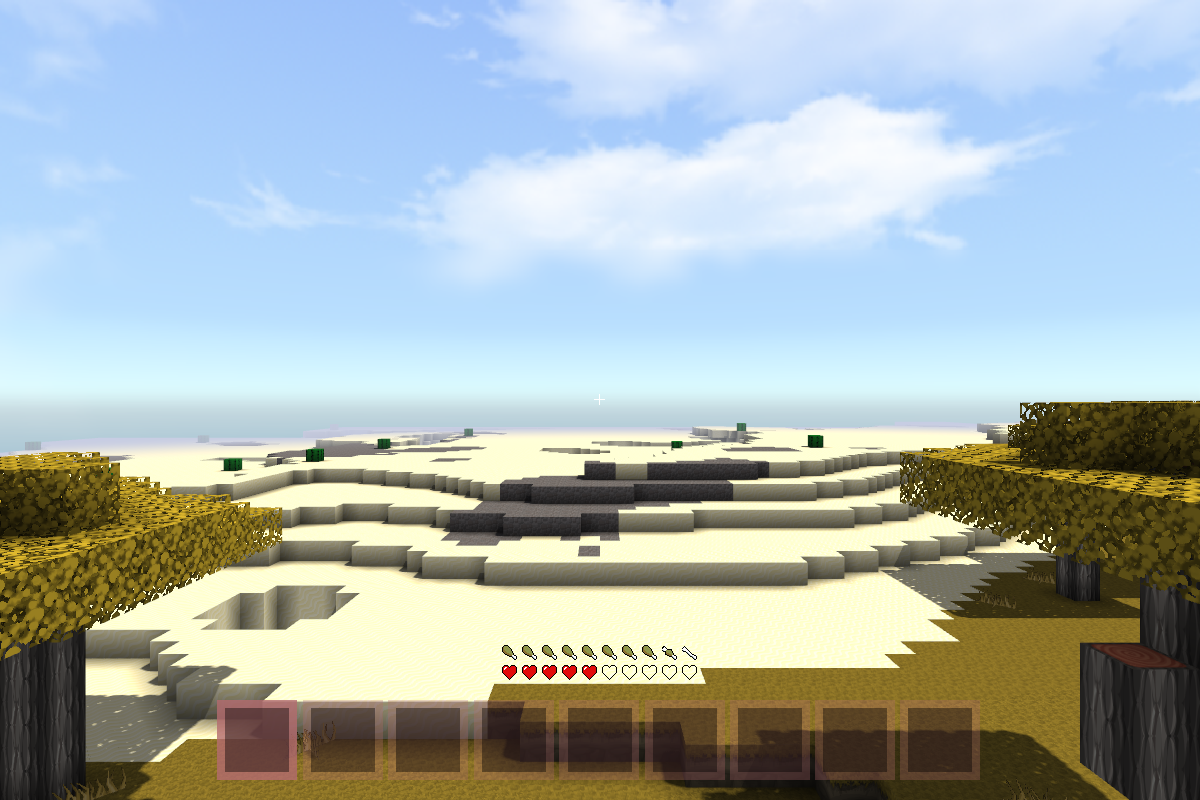
\includegraphics[width=.49\textwidth]{seed-2.png}
	\caption[Von der Terrain-Generierung der Blocklib erzeugte Welten mit unterschiedlichen Seeds.]{Von der Terrain-Generierung der Blocklib erzeugte Welten mit unterschiedlichen Seeds. Links wird der Seed 0 verwendet, rechts der Seed 2. Durch diese kleine Änderung entstehen völlig andere Welten.}\label{fig:static}
\end{figure}
Damit \sysA{} und \sysB{} bei Messungen mit Terrain-Generierung vergleichbar sind, wird in beiden Systemen derselbe Seed verwendet, wodurch dieselbe Welt generiert wird. Abbildung~\ref{fig:static} zeigt zwei Bildschirmfotos von generierten Welten. Das linke Bild zeigt die mit dem Seed $0$ generierte Welt, das rechte Bild nutzt den Seed $2$. Hier sieht man beispielhaft, dass bereits kleine Unterschiede im Seed völlig andere Welten erzeugen. Für die folgenden Messungen wird der Seed $0$ verwendet. 

Im Szenario Welt-Statisch bleibt die Kamera wie in den vorherigen beiden Szenarien an derselben Stelle.



\paragraph{\ac{fps}}

Der Verlauf der \ac{fps} in diesem Szenario ist in Abbildung~\ref{fig:seed-0-static-fps} abgebildet. Vergleicht man die Framerate mit denen der vorherigen Szenarien, lässt sich erkennen, dass sich die Startphase in beiden Systemen verlängert. \sysA{} benötigt 20 Sekunden statt 15 Sekunden, um eine konstante Framerate von etwa \SI{201}{\fps} zu erreichen. \sysB{} erreicht einen stabilen Zustand nach etwa 22 Sekunden mit durchschnittlich \SI{468}{\fps}.

\begin{figure}[!htbp]
	\fpsplot{seed-0-static}
	\caption{Graph des Verlaufs der Framerate in Szenario 3: Welt-Statisch.}\label{fig:seed-0-static-fps}
\end{figure}

Beide Systeme benötigen mit Terrain-Generierung also etwa 5 Sekunden länger für den Start. \sysB{} erreicht nach dem Start eine um \SI{133}{\percent} gesteigerte Framerate gegenüber \sysA{}. Dieser Wert liegt zwischen den gemessenen Werten der ersten beiden Szenarien. Des Weiteren ist liegt die Bildwiederholrate von \sysA{} in diesem Szenario unter der in Szenario 2 gemessenen, während sie in \sysB{} höher liegt.

\paragraph{\ac{cpu}}
Unter Betrachtung der \ac{cpu}-Last im Welt-Statisch Szenario, die in Abbildung~\ref{fig:seed-0-static-cpu} zu sehen ist, lässt sich der zusätzliche Aufwand für die Terrain-Generierung der Welt ebenfalls erkennen.
\begin{figure}[!htbp]
	\cpuplot{seed-0-static}
	\caption[Graph des Verlaufs der \glsentryshort{cpu}-Auslastung in Szenario 3: Welt-Statisch.]{Graph des Verlaufs der \ac{cpu}-Auslastung in Szenario 3: Welt-Statisch.}\label{fig:seed-0-static-cpu}
\end{figure}
Während des Starts der Blocklib lasten beide Systeme die \ac{cpu} bis zu \SI{97}{\percent} aus. Nach dem Start fällt die Auslastung in beiden Systemen, auf durchschnittlich \SI{13}{\percent} in \sysA{} und \SI{23}{\percent} in \sysB{}.
\sysB{} führt im Vergleich zu \sysA{} in diesem Szenario also zu einer um \SI{77}{\percent} erhöhten Last der \ac{cpu}. \sysB{} lastet die \ac{cpu} in diesem Szenario mehr aus als in den Szenarien ohne generierte Welt. \sysA{} dagegen erreicht nach dem Start eine zu den bisherigen Szenarien identische Auslastung.

\paragraph{\ac{gpu}}
Der zeitliche Verlauf der \ac{gpu}-Auslastung von Szenario 3 ist in Abbildung~\ref{fig:seed-0-static-gpu} zu sehen. Die durchschnittliche Last der \ac{gpu} liegt in \sysA{} bei \SI{40}{\percent} und in \sysB{} bei \SI{71}{\percent}. Die Auslastung in \sysA{} entspricht damit der aus dem Hexagon Szenario. \sysB{} dagegen erreicht eine deutlich höhere Last. In beiden Systemen ist die \ac{gpu} noch nicht vollständig ausgelastet. Wie auch in den anderen Messungen zu Szenario 3 zu erkennen ist, zeigt die erst später ansteigende Last der \ac{gpu} eine länger dauernde Startphase an. Die Auslastung beider Systeme bleibt während der Hauptphase weitgehend konstant.
\begin{figure}[!htbp]
	\gpuplot{seed-0-static}
	\caption[Graph des Verlaufs der \glsentryshort{gpu}-Auslastung in Szenario 3: Welt-Statisch.]{Graph des Verlaufs der \ac{gpu}-Auslastung in Szenario 3: Welt-Statisch.}\label{fig:seed-0-static-gpu}
\end{figure}

\paragraph{\ac{ram}}
Die Speichernutzung im Welt-Statisch Szenario ist in beiden Systemen höher als in den vorherigen Szenarien. Abbildung~\ref{fig:seed-0-static-mem} beschreibt deren Verlauf. 
\begin{figure}[!htbp]
	\memplot[xticklabels={,,},xlabel={}]{seed-0-static-multi-mem.csv}{\sysA}
	\\\memplot{seed-0-static-multi-mem.csv}{\sysB}
	\caption{Graph des Verlaufs der Speichernutzung in Szenario 3: Welt-Statisch.}\label{fig:seed-0-static-mem}
\end{figure} 
Wie in Szenario 2 ist die Geschwindigkeit, mit der Speicher für die Erzeugung kurzlebiger Objekte verbraucht wird, in \sysB{} mit \SI{208}{\mega\byte\per\second} etwa doppelt so hoch wie in \sysA{} mit \SI{94}{\mega\byte\per\second}. Allerdings ist die Geschwindigkeit beider Systeme in Szenario 3 insgesamt im Vergleich zu dem Halbwürfel Szenario ungefähr verdoppelt.
Auch der Gesamtverbrauch \ac{ram} ist in beiden Systemen etwa doppelt so groß. \sysA{} nutzt während der Hauptphase \SI{1243}{\mega\byte} und \sysB{} \SI{1793}{\mega\byte} des \ac{ram}. \sysB{} nutzt in diesem Szenario also \SI{44}{\percent} mehr Speicher als \sysA{}.   